\section{Basis expansion and regularisation}
To extend the flexibility of linear model, a transformation of $\X$ can be performed and then use a linear model to the derived input features. Denoting the transformation $h_m(\X) : \CMcal{R}^p\rightarrow \CMcal	{R}$ for a single input $m$, we have the model:
\begin{equation}
f(\X) = \sum_{m=1}^M \beta_mh_m(\X)
\end{equation}
$h()$ are called \textbf{basis function}
Any kind of transformation can be applied: square-roots, squared (on single inputs i.e, $x_i^2$ or among different inputs $x_ix_j$), logarithmic, power functions, trigonometric, etc. 

Polynomials are more widely used but they have a limitation due to its global nature: when tweaking the  parameters to achieve a desired behaviour in a specific region, problems might arise in another region.

A solution is to consider \textbf{piecewise-polynomials} and \textbf{splines}.

\subsection{Piecewise Polynomials and splines}
For the moment $X$ is assumed one-dimensional. A piecewise polynomial function is obtained by  dividing the domain of $X$ into contiguous intervals and use a different $f$ in each interval.

Given a sequence $a=t_0<t_1<\cdots<t_{m+1}=b$, the piecewise polynomials are delimited by an adjacent pair in the sequence. So we have the following sequence of intervals:

\begin{equation}
I_\ell = \left[ t_{\ell-1}, t_\ell\right) \textit{ for } 1\le l\le m \textit{ and } \left[t_m, t_{m+1}\right]
\end{equation}
So the piecewise polynomials, having basis functions: $h_0(X) = 1, h_1(X) = X, h_2(X) = X^2$ and so on, is:

\begin{equation}
f(x) = \left\{ \begin{array}{ll} g_0(x) = \beta_{0,0} + \beta_{0,1} X + \cdots + \beta_{0,k-1} X^{k-1}\quad X \in I_1 \\ 
\vdots\\
 g_{m-1}(x) = \beta_{m-1,0} + \beta_{m-1,1} X + \cdots + \beta_{m-1,k-1} X^{k-1}\quad X \in I_{k+1} \\  \quad 
\end{array}
 \right.
\end{equation}

In this way we get discontinuities at the boundaries. Note that discontinuity means we get completely different values for almost the same input. More often we would like to have continuity at the boundaries or knots: $f(\xi^+)=f(\xi^-)$ which implies the condition:$\beta_1 +\xi\beta_2 = \beta_3 +\xi_1\beta_4$ which removes one degree of freedom.

These constrains, one for each knot, can be embedded in additional basis functions of the type $h(X) = \br{X - \xi}_+$ where $\br{\cdot}_+ = \max(\cdot, 0)$ i.e., the basis function is $0$ for $X - \xi<\xi$, $X - \xi$ otherwise
\begin{equation}
h(X) = \br{X - \xi}_+ = \max(X - \xi, 0) = \left\{ \begin{array}{ll}  0 &\quad X-\xi<0\\
X-\xi &\quad X-\xi\ge0
\end{array}
 \right.
\end{equation}

Using the previous and these basis functions we can reexpress the global function as:
\begin{equation}
\begin{aligned}
f(x) =& \beta_{0,0} + \beta_{0,1}X +\cdots+\beta_{0,k-1}  X^{k-1} + \\
&+\beta_{1,0}(X -\xi_0)_+^0     + \beta_{1,1}(X -\xi_0)_+^1       +\cdots +\beta_{1,k-1} (X -\xi_0)_+^{k-1}+  \\
&+\vdots \\ 
&+\beta_{m-1,0}(X -\xi_{m-1})_+^0 +\cdots +\beta_{m-1,k-1} (X -\xi_{m-2})_+^{k-1}
\end{aligned}
\end{equation}
\textbf{To force continuity between two regions} we set the terms $\beta_{1,0}(X -\xi_j)_+^0$ to $0$:

For example forcing continuity at the first knot:
\begin{equation}
\begin{aligned}
&\beta_{1,0}(X -\xi_0)_+^0 = \beta_{0,0} + \beta_{0,1} \xi_0\\
&\Rightarrow \beta_{1,0} = \beta_{0,0} + \beta_{0,1} \xi_0
\end{aligned}
\end{equation}

 In this way we don't have a jump at the boundaries:

\begin{equation}
\begin{aligned}
f(x) =& \beta_{0,0} + \beta_{0,1}X +\cdots+\beta_{0,k-1}  X^{k-1} + \\
&+ \beta_{1,1}(X -\xi_0)_+^1       +\cdots +\beta_{1,k-1} (X -\xi_0)_+^{k-1}+  \\
&+\vdots \\ 
&+ \beta_{m-1,1}(X -\xi_{m-1})_+^1 +\cdots +\beta_{m-1,k-1} (X -\xi_{m-1})_+^{k-1}
\end{aligned}
\end{equation}
In this way we have removed $m-1$ parameters.

There is a difference in this representation: before we have to select a polynomial function for a specific region where the fit to the global function was given by the fit of the parameters specific to that region, now we have a global function that works a little differently. In the first region, the only non-null terms are $\beta_{0,j}$ as before. When reaching the second region, the terms $\beta_{1,j}$ becomes non-null. Now the coefficients of the polynomial are the sum of the coefficients of these two region: i.e., in the second region we have:
\begin{equation}
\begin{aligned}
f(x) =& \beta_{0,0} -(\beta_{1,1}+\cdots+\beta_{1,k-1})\xi_0+ (\beta_{0,1}+\beta_{1,1})X+\\
&+\cdots+(\beta_{0,k-1}  +\beta_{1,k-1})X^{k-1}
\end{aligned}
\end{equation}

\autoref{spline_linear} shows the global function, solid line, given by the sum of basis functions, dashed lines, when traversing the graph from left to right. At each knot, a new basis function is activated and summed to the global function.

The basis functions can be seen as a correction to the global polynomial for that  specifc region and the knots are those points where the correction starts. At the knot $X=\xi_j$ so the correction starts very gently and the continuity is preserved.

\begin{figure}
\begin{subfigure}{0.49\textwidth}
\centering
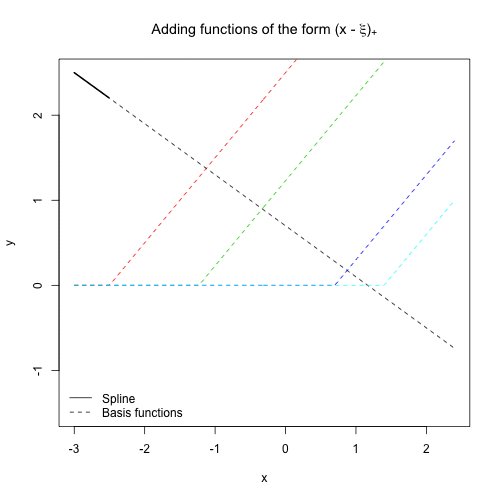
\includegraphics[width=0.9\linewidth]{img/spline_linear/10}
\caption{First region.}
\end{subfigure}
\hfill
\begin{subfigure}{0.49\textwidth}
\centering
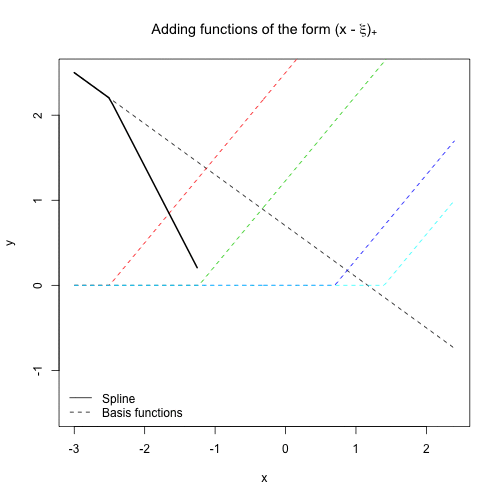
\includegraphics[width=0.9\linewidth]{img/spline_linear/33}
\caption{Second region.}
\end{subfigure}
\begin{subfigure}{0.49\textwidth}
\centering
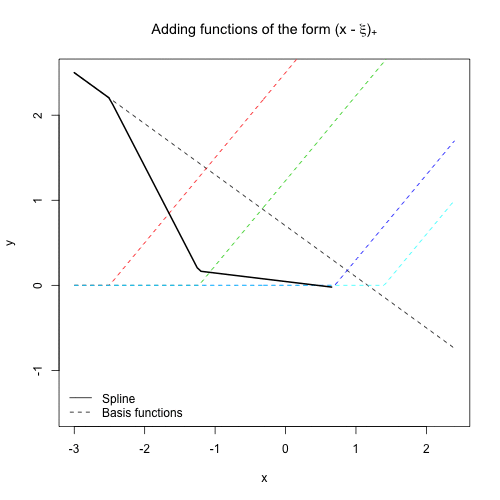
\includegraphics[width=0.9\linewidth]{img/spline_linear/68}
\caption{Third region.}
\end{subfigure}
\hfill
\begin{subfigure}{0.49\textwidth}
\centering
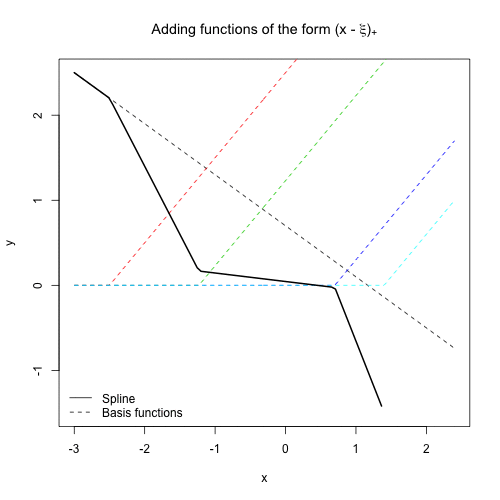
\includegraphics[width=1\linewidth]{img/spline_linear/81}
\caption{Fourth region.}
\end{subfigure}
\end{figure}
\begin{figure}\ContinuedFloat
\begin{subfigure}{0.49\textwidth}
\centering
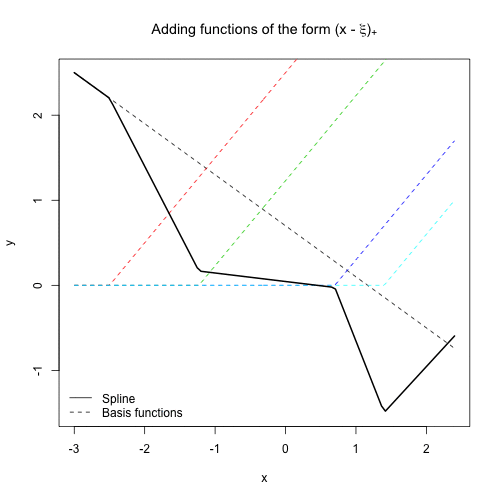
\includegraphics[width=1\linewidth]{img/spline_linear/100}
\caption{Fifth region.}
\end{subfigure}
\caption{Linear splines. The solid line is the global function while the dashed lines are the basis functions.}
\label{spline_linear}
\end{figure}

Generally, smoother functions are preferred and these are achieved by increasing the order of the local polynomials and increasing the order of continuity (continuity first derivative, second derivative). It is claimed that cubic splines are the lowest-order spline for which the discontinuity is not visible to the human eye and seldom higher degrees are needed, unless smooth derivatives are required.

The spline order, number of knots and their positions must be selected. Generally the position of the knots is chosen according the observation, while the order is chosen a-priori.

\begin{figure}
\begin{subfigure}{0.49\textwidth}
\centering
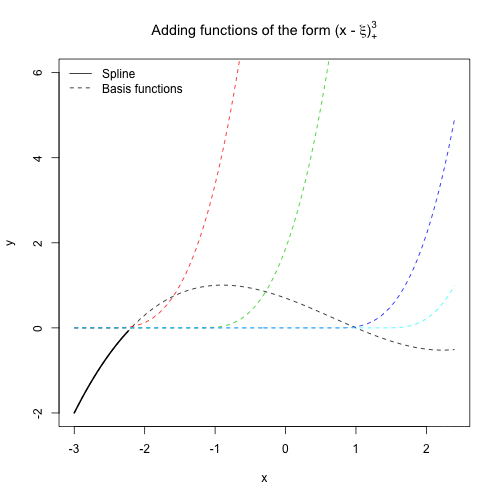
\includegraphics[width=1\linewidth]{img/spline_cubic/15}
\caption{First region.}
\end{subfigure}
\hfill
\begin{subfigure}{0.49\textwidth}
\centering
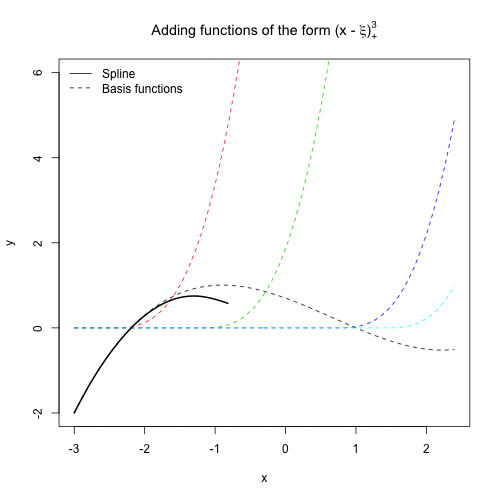
\includegraphics[width=1\linewidth]{img/spline_cubic/41}
\caption{Second region.}
\end{subfigure}
\begin{subfigure}{0.49\textwidth}
\centering
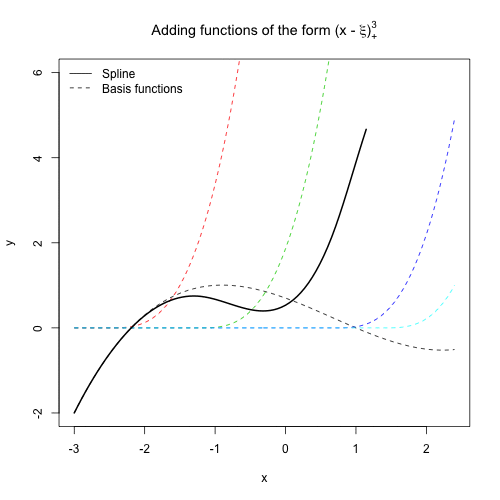
\includegraphics[width=1\linewidth]{img/spline_cubic/77}
\caption{Third region.}
\end{subfigure}
\hfill
\begin{subfigure}{0.49\textwidth}
\centering
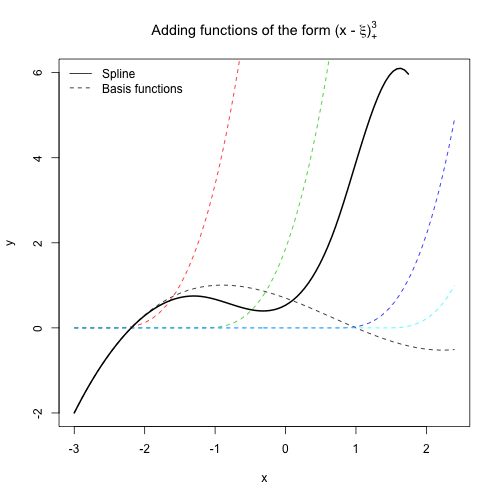
\includegraphics[width=1\linewidth]{img/spline_cubic/88}
\caption{Fourth region.}
\end{subfigure}
\end{figure}
\begin{figure}\ContinuedFloat
\begin{subfigure}{0.49\textwidth}
\centering
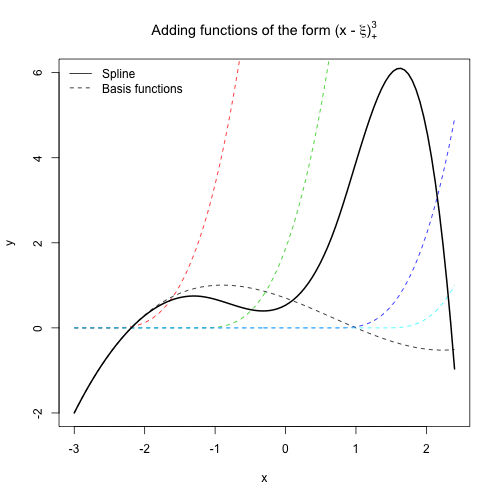
\includegraphics[width=1\linewidth]{img/spline_cubic/100}
\caption{Fifth region.}
\end{subfigure}
\label{spline_cubic}
\caption{Cubic splines. The solid line is the global function while the dashed lines are the basis functions.}
\end{figure}

\subsection{Natural cubic splines}
Polynomial fits to data tends to be erratic at the boundaries and additionally splines behave even more widely than the global polynomial beyond the boundaries. This is shown by the point-wise variance (the variance of the estimator at one point: $\Var[\hat{f}(x_0)]$ in \autoref{pointwise_var}. Note the variance explosion close to the boundaries, especially for cubic splines.

\begin{figure}
\centering
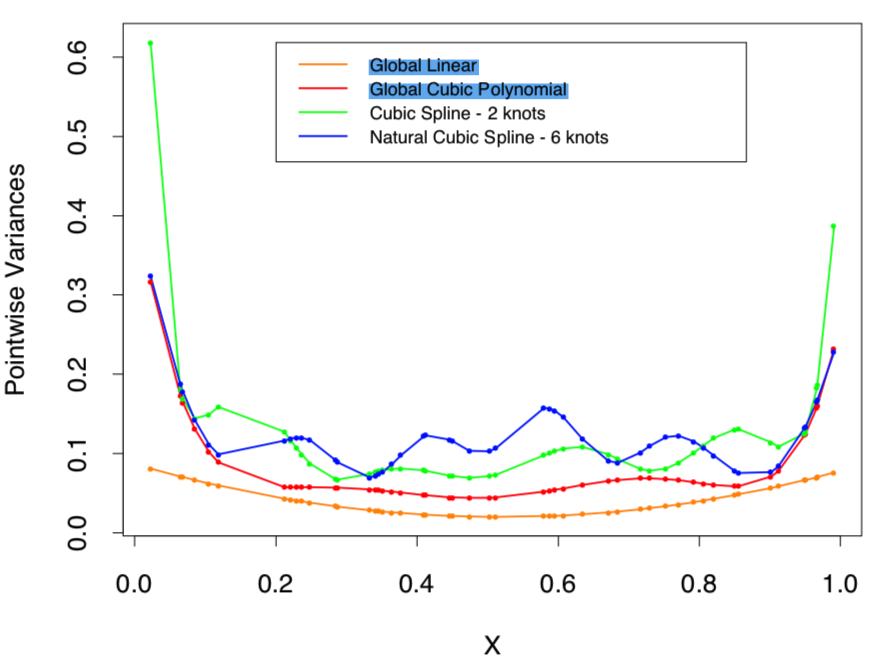
\includegraphics[scale=0.4]{img/pointwise_var}
\caption{$X$ consists of 50 points drawn randomly from $U[0,1]$ and an assumed error model of with constant variance. Both cubic splines have 6 degrees of freedom. The cubic spline has two knots at $0.33$ and at $0.66$ while the natural cubic spline has boundary knots at $0.1$ and $0.9$, and four interior knots uniformly spaced between them.}
\label{pointwise_var}
\end{figure}

A  \textbf{natural cubic spline} adds additional constraints by forcing linearity beyond the boundary knots. These frees up four degrees of freedom (2 in both boundary regions), that can be used more profitably by sprinkling more knots in the interior region. There will be a price to pay in terms of bias near the boundaries, but in these regions we have less information anyway so assuming the function is linear here is reasonable.

A natural cubic spline with $K$ knots is represented by $K$ basis functions. One can start from the basis of a cubic spline and then derive the reduce basis by imposing the boundary constraints.

Starting from the general continuous basis for four regions (four knots):
\begin{equation}
\begin{aligned}
&h_1(X) =1, \quad\quad\quad h_2(X) =X,\quad h_3(X) =X^2,\quad  h_4(X) = X^3,\\
&h_5(X) = X-\xi_0,\quad h_6(X) = (X-\xi_0)^2,\quad, h_7(X) = (X-\xi_0)^3\\
&h_8(X) = X-\xi_1,\quad h_9(X) = (X-\xi_1)^2,\quad h_{10}(X) = (X-\xi_1)^3\\
&h_9(X) = X-\xi_2,\quad h_10(X) = (X-\xi_1)^2,\quad h_{11}(X) = (X-\xi_2)^3
\end{aligned}
\end{equation}
Enforcing also continuity of the first and second derivatives at the knots we reduce the basis to:
\begin{equation}
\begin{aligned}
&h_1(X) = 1, \quad h_2(X) =X,\quad h_3(X) =X^2,\quad  h_4(X) = X^3,\\
&h_5(X) = (X-\xi_0)^3, \quad h_6(X) = (X-\xi_1)^3, \quad h_7(X) = (X-\xi_2)^3.
\end{aligned}
\end{equation}

Enforcing linearity beyond the boundaries, we eliminate $ h_3(X)$ and $ h_4(X)$. We must also keep the cubic expression in the intermediate regions but somehow make the cubic part cancel out when reaching the fifth region since here it must be linear. We can add for each region in the interval $[1, K-2]$ the following basis function:
\begin{equation}
\begin{aligned}
&h_k(X) = d_k(X) - d_{K-1}(X)\\
\textit{where} \quad &d_k(X) = \frac{\br{X-\xi_k}_+^3 - \br{X-\xi_K}_+^3 }{\xi_K - \xi_k}
\end{aligned}
\end{equation}

In the first region we have:
\begin{equation}
\hat{f}_1(X) = \beta_0 + \beta_1 X
\end{equation}
In the second region we have:
\begin{equation}
\begin{aligned}
&\hat{f}_2(X) = \beta_0 + \beta_1 X +\beta_2 \frac{(X-\xi_0)^3}{\xi_2 - \xi_0} =\\
&= \beta_0 + \beta_1 X +\beta_2 \frac{X^3 -3 \xi_0 X^2 + 3\xi_0^2 X-\xi_0^3}{\xi_2 - \xi_0} =\\
&= \frac{\beta_2}{\xi_2 - \xi_0} X^3 -3 \beta_2\frac{\xi_0}{\xi_2 - \xi_0} X^2 + (\beta_1+3\beta_2\frac{\xi_0^2}{\xi_2 - \xi_0})X + \beta_0 - \beta_2\frac{\xi_0^3}{\xi_2 - \xi_0}
\end{aligned}
\end{equation}
In the third region we have:
\begin{equation}
\begin{aligned}
&\hat{f}_3(X) = \beta_0 + \beta_1 X  +\beta_2 h_2(X) = \beta_0 + \beta_1 X  +\beta_2\left[ \frac{(X-\xi_0)^3}{\xi_2 - \xi_0} - \frac{(X-\xi_1)^3}{\xi_2 - \xi_1}\right]  \\
&= \beta_0 + \beta_1 X +\beta_2 \left[ \frac{X^3 -3 \xi_0 X^2 + 3\xi_0^2 X-\xi_0^3}{\xi_2 - \xi_0} -  \frac{X^3 -3 \xi_1 X^2 + 3\xi_1^2 X-\xi_1^3}{\xi_2 - \xi_1}\right] =\\
&= \beta_0 + \beta_1 X +\beta_2 \frac{(\xi_2-\xi_1-\xi_2+\xi_0)X^3-3\left[ \xi_0(\xi_2-\xi_1) - \xi_1(\xi_2-\xi_0)\right]X^2}{(\xi_2 - \xi_0)(\xi_2 - \xi_1)}+\\
&\quad +  \frac{3\left[\xi_0^2(\xi_2-\xi_1) - \xi_1^2(\xi_2-\xi_0) \right]X-\left[(\xi_0^3(\xi_2-\xi_1) -\xi_1^3(\xi_2-\xi_0)\right]}{(\xi_2 - \xi_0)(\xi_2 - \xi_1)}=\\
&=  \beta_0 + \beta_1 X +\beta_2 \frac{(-\xi_1+\xi_0)X^3-3\xi_2(\xi_0-\xi_1)X^2}{(\xi_2 - \xi_0)(\xi_2 - \xi_1)}+\\
&\quad +  \frac{3\left[\xi_2(\xi_0-\xi_1)(\xi_0+\xi_1)-\xi_0\xi_1(\xi_0-\xi1)\right]X}{(\xi_2 - \xi_0)(\xi_2 - \xi_1)}+\\
&\quad\quad-\frac{\left[\xi_2(\xi_0-\xi_1)(\xi_0^2-\xi_0\xi_1+\xi_1^2)-\xi_0\xi_1(\xi_0-\xi1)(\xi_0+\xi_1)\right]}{(\xi_2 - \xi_0)(\xi_2 - \xi_1)} = \\
&=\beta_0 + \beta_1 X -\beta_2 (\xi_1-\xi_0)\frac{X^3-3\xi_2X^2}{(\xi_2 - \xi_0)(\xi_2 - \xi_1)}+\\
&\quad\quad +  \frac{3\left[\xi_2(\xi_0+\xi_1)-\xi_0\xi_1\right]X-\left[\xi_2(\xi_0^2-\xi_0\xi_1+\xi_1^2)-\xi_0\xi_1(\xi_0+\xi_1)\right]}{(\xi_2 - \xi_0)(\xi_2 - \xi_1)}=\\
&= -\beta_2\frac{(\xi_1-\xi_0)}{(\xi_2 - \xi_0)(\xi_2 - \xi_1)} X^3 +3 \beta_2\frac{\xi_2(\xi_1-\xi_0)}{(\xi_2 - \xi_0)(\xi_2 - \xi_1)} X^2 + \\
&\quad\quad +(\beta_1-3\beta_2(\xi_1-\xi_0)\frac{\xi_2(\xi_0+\xi_1)-\xi_0\xi_1}{(\xi_2 - \xi_0)(\xi_2 - \xi_1)})X +\\
&\quad\quad+ \beta_0 + \beta_2(\xi_1-\xi_0)\frac{\xi_2(\xi_0^2-\xi_0\xi_1+\xi_1^2)-\xi_0\xi_1(\xi_0+\xi_1)}{(\xi_2 - \xi_0)(\xi_2 - \xi_1)}
\end{aligned}
\end{equation}
In the fourth region:
\begin{equation}
\begin{aligned}
&\hat{f}_3(X) = \beta_0 + \beta_1 X  +\beta_2 h_2(X) =\\
&= \beta_0 + \beta_1 X  +\beta_2\left[ \frac{(X-\xi_0)^3-(X-\xi_2)^3}{\xi_2 - \xi_0} - \frac{(X-\xi_1)^3-(X-\xi_2)^3}{\xi_2 - \xi_1}\right]  \\
&= \beta_0 + \beta_1 X +\beta_2 \frac{X^3 -3 \xi_0 X^2 + 3\xi_0^2 X-\xi_0^3-X^3 +3 \xi_2 X^2 - 3\xi_2^2 X+\xi_2^3}{\xi_2 - \xi_0} +\\
&\quad\quad\quad -\beta_2  \frac{X^3 -3 \xi_1 X^2 + 3\xi_1^2 X-\xi_1^3-X^3 +3 \xi_2 X^2 - 3\xi_2^2 X+\xi_2^3}{\xi_2 - \xi_1} =\\
&= \beta_0 + \beta_1 X +\beta_2 \frac{ 3 (\xi_2-\xi_0) X^2 - 3(\xi_2^2- \xi_0^2) X+\xi_2^3-\xi_0^3}{\xi_2 - \xi_0} +\\
&\quad\quad\quad -\beta_2         \frac{3 (\xi_2-\xi_1 ) X^2 - 3(\xi_2^2 - \xi_1^2) X+\xi_2^3-\xi_1^3  }{\xi_2 - \xi_1} =\\
&= \beta_0 + \beta_1 X +\beta_2 \frac{ \cancel{3(\xi_2 - \xi_1) (\xi_2-\xi_0) X^2} - 3(\xi_2 - \xi_1)(\xi_2^2- \xi_0^2) X+(\xi_2 - \xi_1)(\xi_2^3-\xi_0^3)}{(\xi_2 - \xi_0)(\xi_2 - \xi_1)} +\\
&\quad\quad\quad -\beta_2         \frac{\cancel{3 (\xi_2 - \xi_0)(\xi_2-\xi_1 ) X^2} - 3(\xi_2 - \xi_0)(\xi_2^2 - \xi_1^2) X+(\xi_2 - \xi_0)(\xi_2^3-\xi_1^3  )}{(\xi_2 - \xi_0)(\xi_2 - \xi_1)} =\\
&= \beta_0 + \beta_1 X +\beta_2 \frac{- 3(\xi_2 - \xi_1)(\xi_2^2- \xi_0^2) X+(\xi_2 - \xi_1)(\xi_2^3-\xi_0^3)}{(\xi_2 - \xi_0)(\xi_2 - \xi_1)} +\\
&\quad\quad\quad -\beta_2         \frac{- 3(\xi_2 - \xi_0)(\xi_2^2 - \xi_1^2) X+(\xi_2 - \xi_0)(\xi_2^3-\xi_1^3  )}{(\xi_2 - \xi_0)(\xi_2 - \xi_1)} =\\
&= \beta_0 + \beta_1 X +\beta_2 \frac{3\left[-\xi_2(\xi_1^2-\xi_0^2)+\xi_2^2(\xi_1-\xi_0)+\xi_0\xi_1(\xi_1-\xi_0)\right]X+}{(\xi_2 - \xi_0)(\xi_2 - \xi_1)}\\
&\quad\quad \frac{-\xi_2(\xi_1^3-\xi_0^3)-\xi_2^3(\xi_1-\xi_0)-\xi_0\xi_1(\xi_1-\xi_0)}{(\xi_2 - \xi_0)(\xi_2 - \xi_1)}
\end{aligned}
\end{equation}
Note that the fourth region is linear.
\subsection{Smoothing splines}
We can avoid knot selection by using a maximal set of knots, controlled by a regularization process. The problem is: \textit{Among all functions $f(x)$ with two continuous derivatives, find the one that minimizes the penalized residual sum of squares}:
\begin{equation}
RSS(f,\lambda) = \sum_{i=1}^N \left[y_i - f(x_i)\right]^2 + \lambda \int f''(t) dt
\label{RSSspl}
\end{equation}
The first term measures closeness to the data, while the second term penalizes curvature in the function. If $\lambda=0$ $f$ can be any function that interpolates the data so we can achieve smoothness. If $\lambda=\infty$ simple least squares line fit, since no second derivative can be tolerated and we get a "rough" function.
\autoref{RSSspl} has an explicit finite-dimensional unique minimizer which is a natural cubic spline with knots at the unique values of the $x_i$, $i = 1,...,N$, so there are as many as $N$ knots, hence $N$ degrees of freedom. The penalty translates to a penalty on the spline coefficients, which are shrunk to the linear fit.

Being the solution a natural spline, we can write it as:
\begin{equation}
f(x) = \sum_{j=1}^N N_j(x)\theta_j
\end{equation}
where $N_j(x)$ are the N-dimensional set of basis functions for representing this family of natural splines:
\begin{equation}
RSS(\theta, \lambda) = \br{\y - \mathbf{N}\theta}^T\br{\y - \mathbf{N}\theta}+\lambda \theta^T\mathbf{\Sigma_N}\theta
\end{equation}
where ${N}_{i,j} = N_j(x_i)$ and $${\mathbf{\Sigma_N}}_{j,k} = \int N_j''(t)N_k''(t)dt$$. The solution is :
\begin{equation}
\hat{\theta} = \br{\mathbf{N}^T\mathbf{N}+\lambda\mathbf{\Sigma}_N}^{-1}\mathbf{N}^T\y = \mathbf{S_\lambda} \y
\end{equation}
which is a generalized ridge regression. $\mathbf{S_\lambda}$ is positive-definite, symmetric and $\mathbf{S_\lambda}\mathbf{S_\lambda} \le \mathbf{S_\lambda}$. Since it is symmetric and positive-definite it has a real eigenvalue decomposition. Let us re-write $\mathbf{S_\lambda} = \br{\I-\lambda \mathbf{K}}^{-1}$.
The eigenvalue decomposition of $\mathbf{S_\lambda}$ is:
\begin{equation}
\begin{aligned}
\mathbf{S_\lambda} = \sum_{k=1}^N \rho_k(\lambda)\mathbf{u}_k\mathbf{u}_k^T\\
\rho_k(\lambda) = \frac{1}{1+\lambda d_k}
\end{aligned}
\end{equation}
The degrees of freedom are $df_\lambda = Tr(\mathbf{S_\lambda})$.

The eigenvectors are not affected by changes in $\lambda$, and hence the whole family of smoothing splines for a particular sequence of $x$, indexed by $\lambda$ have the same eigenvectors.
$\mathbf{S_\lambda} \y= \sum_{k=1}^N \mathbf{u}_k\rho_k(\lambda)\langle\mathbf{u}_k,\y\rangle$: the smoothing spline decomposes $\y$ w.r.t. the complete basis $\mathbf{u}_k$ and differently shrinking the contributions using $\rho_k(\lambda)$. 
So for example suppose $\mathbf{B}_xi$ is a matrix of cubic-splines basis functions. Then the vector of fitted spline values is given by $\hat{f} = \mathbf{B}_\xi (\mathbf{B}_\xi^T\mathbf{B}_\xi)^{-1} \mathbf{B}_\xi^T\y = \mathbf{H}_\xi \y$.In such a basis regression method the contributions are either left alone or shrunk to $0$. The first two eigenvalues are always $1$ and they correspond to the two-dimensional eigenspace of functions linear in $x$ which are never shrunk. The eigenvalues $\rho_k(\lambda) = 1/(1 + \lambda dk)$ are an inverse function of the eigenvalues $d_k$ of the penalty matrix $\mathbf{K}$, moderated by $\lambda$; $\lambda$ controls the rate at which the $\rho_k(\lambda)$ decrease to zero. $d1 = d2 = 0$ and again linear functions are not penalized.

\subsection{Multidimensional splines}
Suppose $X \in \CMcal{R}^2$ and suppose we have two sets: $h_{1,k}(X_1), k=1,\cdots, M_1$ for representing functions of coordinate $X_1$, and a set of $M_2$ functions $h_{2,k}(X_2)$ for coordinate $X_2$. Then the$M_1\times M_2$ dimensional tensor product basis defined by:
\begin{equation}
g_{j,k} = h_{1,j}(X_1)h_{2,k}(X_2), \quad j=1,\cdots, M_1, \quad k=1,\cdots, M_2 
\end{equation}
can be used for representing a two-dimensional function:
\begin{equation}
g(X) = \sum_{j=1}^{M_1}\sum_{k=1}^{M_2} \theta_{jk}g_{jk}(X)
\end{equation}

The coefficients can be fit with least squares. This can be generalized to d dimensions, but note that the dimension of the basis grows exponentially fast.

One-dimensional smoothing splines (via regularization) generalize to higher dimensions as well. Suppose we have pairs $y_i,x_i$ with $x_i \in \CMcal{R}^d$, and we seek a d-dimensional regression function $f(x)$. The idea is to set up the problem:
\begin{equation}
min_f \sum_{i=1}^N \left[y_i - f(x_i)\right]^2 +\lambda J\left[f\right]
\end{equation}
where $J$ is an appropriate penalty functional for stabilizing a function f in $\CMcal{R}^d$. For example:
\begin{equation}
 J\left[f\right] = \int \int_{\CMcal{R}^2} \left[ \left( \frac{\partial^2 f(x)}{\partial x_1^2} \right)^2+2\left(\frac{\partial^2 f(x)}{\partial x_1 \partial x_2} \right)^2+\left(\frac{\partial^2 f(x)}{\partial x_2^2} \right)^2\right]dx_1dx_2
\end{equation}
If $\lambda\rightarrow 0$ the solution approaches an interpolating function, as $\lambda$ the solution approaches the least squares plane.
The solution has the form:
\begin{equation}
f(x) = \beta_0 + \beta^T x + \sum^N_{j=1} \alpha_j h_j(x)
\end{equation}

Additive spline model can be represented in this formulation too: there exists a penalty $J[f]$ that guarantees that the solution has the from $f(X) = \alpha + f_1(X_1) +\cdots + f_d(X_d)$ and that each of the functions $f_j$ are univariate splines. In this case it is better to assume $f$ is additive and impose an additional penalty and impose an additional penalty on each of the component functions:
\begin{equation}
\begin{aligned}
J[f] = J[f_1+f_2+\cdots+f_d) =\sum_{j=1}^d \int f_j''(t_j)dt_j
\end{aligned}
\end{equation}
These are naturally extended to ANOVA spline decomposition:
\begin{equation}
f(X) = \alpha + \sum_j f_j(X_j) + \sum_{j<k} f_{jk(X_j, X_k}+ \cdots
\end{equation}
where each of the components are splines of the required dimension. There are many choices to be made:
\begin{itemize}
\item maximum order of interaction (the one above is up to order 2);
\item which term to include
\item the representation to use (regression splines with a small number of basis functions and their tensor product for interaction or a complete basis as in smoothing splines and include appropriate regularizers for each term in the expansion.
\end{itemize}

When the number of potential dimensions is large automatic methods are desirable (for example MARS and MART procedures).
\subsection{Wavelet smoothing}
$\cdots$
